\documentclass[tikz,border=2pt,11pt]{standalone}
\usetikzlibrary{positioning}
\usetikzlibrary{arrows.meta}
\usepackage{amsmath}
\usepackage{amssymb}
\usepackage{tikz}
\newcommand{\R}{\mathbb R}
\newcommand{\C}{\mathbb C}
\newcommand{\N}{\mathbb N}
\newcommand{\Q}{\mathbb Q}
\DeclareMathOperator{\dist}{dist}
\DeclareMathOperator{\supp}{supp}
\DeclareMathOperator{\dens}{dens}
\DeclareMathOperator{\ran}{ran}
\DeclareMathOperator{\absconv}{absconv}
\newcommand{\clspan}[1]{\overline{\operatorname{span}}\{#1\}}
\newcommand{\SQ}{\mathrm{SQ}}
\begin{document}
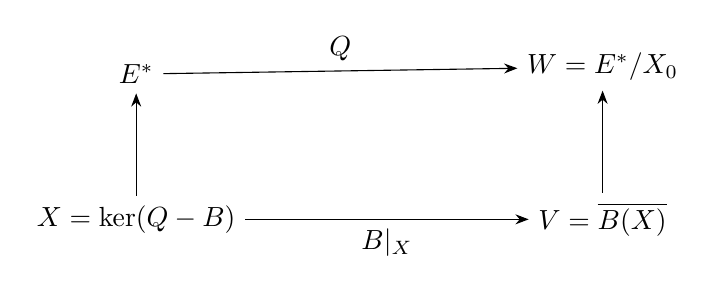
\begin{tikzpicture}[>=Stealth,node distance=13mm and 36mm]
\node (x) {$X=\ker(Q-B)$};
\node[right=of x] (v) {$V=\overline{B(X)}$};
\node[above=of x] (e) {$E^*$};
\node[above=of v] (w) {$W=E^*/X_0$};
\draw[->] (e) -- node[above] {$Q$} (w);
\draw[->] (x) -- node[below] {$B|_X$} (v);
\draw[->] (x) -- (e);
\draw[->] (v) -- (w);
\end{tikzpicture}
\end{document}
